\documentclass[9pt,addpoints]{exam}
\usepackage{enumitem}
\usepackage{amsfonts,amssymb,amsmath, amsthm}
\usepackage{graphicx}
\usepackage{systeme}
\usepackage{pgf,tikz,pgfplots}
\pgfplotsset{compat=1.15}
\usepgfplotslibrary{fillbetween}
\usepackage{mathrsfs}
\usetikzlibrary{arrows}
\usetikzlibrary{calc}
\pagestyle{headandfoot}
%\firstpageheadrule
\runningheader{Homework 1 Solution}{}{Page \thepage\ of \numpages}
\runningheadrule
\author{Aaron GK}
\usepackage{geometry}
\geometry{
	a4paper,
	total={170mm,257mm},
	left=10mm,
	right=10mm,
	bottom=5mm,
	top=5mm,
}
\firstpagefooter{}{}{}
\runningfooter{}{}{}


\begin{document}
	\title{St John Baptist De La Salle Catholic School, Addis Ababa\\
		\large Homework 1 \\
		2nd Quarter}
	\maketitle
	\begin{center}
		\fbox{\fbox{\parbox{6in}{\centering
					Notes, and use of other aids is allowed.  Read all directions carefully and write your answers in the space provided.  To receive full credit, you must show all of your work. \textbf{Cheating or indications of cheating and similar answers will be punished accordingly}. 
		}}}
		\subsubsection*{Information}
		\begin{itemize}
			\item The homework is due on \textbf{Monday}, \textbf{December 5th}.
			\item You should Work on it \textbf{individually} and consult me if you have any questions. As I have reiterated multiple times, cheating will have a serious consequence.
			\item For purposes of neatness and simplicity of grading, you should do the homework on an \textbf{A-4 paper}.
		\end{itemize}
	\end{center}
	\begin{center}
		\subsection*{Questions}
	\end{center}
	
	\begin{questions}
		\subsubsection*{Conceptual Problems}
		\question We do have a great deal of relationship between rotational and translational physical quantities. List the translational equivalents for the following rotational physical quantities: \textit{torque, angular momentum, moment of inertia} and \textit{angular impulse}. \\ \\
		\textbf{Solution}
		\begin{itemize}
			\item Torque is related to force
			\item Angular momentum is related to linear momentum
			\item Moment of inertia is related to mass
			\item Angular impulse is related to impulse
		\end{itemize}
		\question When there is a global heating trend on Earth, the atmosphere expands and the length of the day increases very slightly. Explain why the length of a day increases. \\ \\
		\textbf{Solution} \\
		When there is a global heating trend, the surface of the Earth slightly expands causing the radius of the Earth to grow slightly larger. When the radius is larger, we do have a greater moment of inertia. Assuming the angular momentum is conserved since there is minimal net effect causing this, we can assume the angular speed of the Earth about its own axis to decrease. That means, the time needed to complete a revolution increases. Mathematically:
		$$L_f=L_i(\textit{since angular momentum is conserved})\text{  and  }I_i\lessapprox I_f$$
		$$\text{Since }I_i\lessapprox I_f\text{, we get   }\omega_f\lessapprox\omega_i$$
		$$\text{Since }\omega_f\lessapprox\omega_i,\text{ we can deduce that }\text{T}_i\lessapprox\text{T}_f$$
		\question A point mass is going down an inclined plane. It also rotates while going down the inclined plane - we can deduce that the point mass has both a \textbf{translational}(\textit{linear}) and \textbf{rotational} kinetic energy. What percentage of the total kinetic energy is the rotational kinetic energy? (Assume the moment of inertia of a point mass is $\text{mr}^2$) \\ \\
		\textbf{Solution} \\
		The total kinetic energy of a body is the sum of its rotational and translational kinetic energies. Mathematically,
		$$\text{K}_{\text{tot}}=\text{K}_{\text{trans}}+\text{K}_{\text{rot}}$$
		$$\text{K}_{\text{tot}}=\dfrac{1}{2}\text{mv}^2+\dfrac{1}{2}\text{I}\omega^2$$
		We know that the moment of inertia of a point mass is given by $\text{I}=\text{mr}^2$, thus:
		$$\text{K}_{\text{tot}}=\dfrac{1}{2}\text{mv}^2+\dfrac{1}{2}(\text{mr}^2)\omega^2$$ 
		$$\text{K}_{\text{tot}}=\dfrac{1}{2}\text{mv}^2+\dfrac{1}{2}\text{m}(\text{r}^2\omega^2)$$
		We also know that $\text{rw}=v$, thus $\text{r}^2\omega^2=v^2$. Thus we have:
		$$\text{K}_{\text{tot}}=\dfrac{1}{2}\text{mv}^2+\dfrac{1}{2}\text{mv}^2$$
		$$\text{K}_{\text{tot}}=\text{mv}^2$$	
		We have seen that the rotational kinetic energy for a point mass is $\dfrac{1}{2}\text{I}\omega^2=\dfrac{1}{2}\text{mv}^2$. The percentage is then:
		$$\dfrac{\dfrac{1}{2}\text{mv}^2}{\text{mv}^2}=0.5\approx50\%$$
		\question A uniform 4.0-m plank weighing 200.0 N rests against the corner of a wall, as shown below. There is no friction at the point where the plank meets the corner. (a) Find the forces that the corner and the floor exert on the plank. (b) What is the minimum coefficient of static friction between the floor and the plank to prevent the plank from slipping?
		\begin{center}
			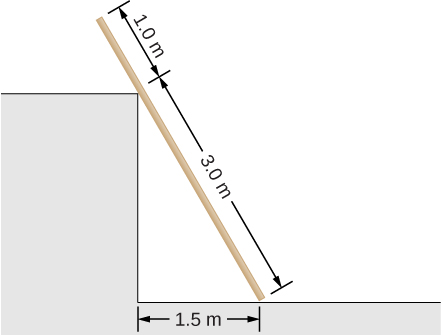
\includegraphics[scale=0.8]{ladder.jpeg}
		\end{center} 
		\textbf{Solution} \\
		For the object to be in equilibrium, forces and torques need to be balanced. To find the balance, we need to first list out all the forces we have acting on the plank: 
		\begin{itemize}
			\item W - the weight of the plank acting 2m away from the point of contact with the ground (\textit{acts along the y-axis})
			\item $\text{F}_1$- the normal force against the plank from the ground (\textit{acts along the y-axis})
			\item $\text{F}_2$- the normal force against the plank from the corner of the wall (\textit{acts along the x-axis})
			\item f - the frictional force that keeps the plank from moving away. (\textit{acts along the x-axis})
		\end{itemize}
		Since our forces need to cancel out for the object to be in equilibrium, we need to add them according to the axes on which the forces are acting.
		$$\sum\text{F}_x=0 \text{    }\&\text{    }\sum \text{F}_y=0 $$
		$$\text{F}_2-f=0\text{    }\&\text{    }\text{F}_1-\text{W}=0$$
		$$\text{F}_2=f\text{    }\&\text{    }\text{F}_1=\text{W}$$
		The value of W is known, hence we can infer the value of $\text{F}_1$. To find the value of $F_2$, we need to use the second condition for equilibrium -- that the net torque on the plank is 0. We have two turning effects - one from the weight(W) and another one from the force on the corner of the wall($\text{F}_2$). Since our axis of rotation is the point of contact between the ground and the plank, the weight causes a counter-clockwise(CCW) torque while the normal force causes a clockwise(CW) one. Hence, we get the following:
		$$\tau_{\text{cw}}=\text{F}_2\times3\text{m}\times\sin(120^0)$$
		$$\tau_{\text{ccw}}=\text{W}\times2.0\text{m}\times\sin(30^0)$$
		Since our plank is in equilibrium, the CW \& CCW torques are equal. Thus:
		$$\text{F}_2\times3\text{m}\times\sin(120^0)=\text{W}\times2.0\text{m}\times\sin(30^0)$$
		$$\text{F}_2=\dfrac{\text{W}\times2.0\text{m}\times\sin(30^0)}{3\text{m}\times\sin(120^0)}=\dfrac{200\text{N}\times2.0\text{m}\times\sin(30^0)}{3\text{m}\times\sin(120^0)}$$
		$$\text{F}_2=\dfrac{400}{3\sqrt{3}}\text{N}$$ \\ \\
		We know that $f=\text{F}_2=\dfrac{400}{3\sqrt{3}}\text{N}$, thus to find our coefficient of friction, we can use this:
		$$f=\mu\text{F}_1\text{, but }f=\text{F}_2\text{. Thus,}$$
		$$\text{F}_2=\mu\text{F}_1$$
		$$\mu=\dfrac{\text{F}_2}{\text{F}_1}=\dfrac{\frac{400}{3\sqrt{3}}\text{N}}{200\text{N}}=\dfrac{2}{3\sqrt{3}}$$
		\question A constant torque is applied to a rotating object whose moment of inertia is  16 kgm$^2$ around the axis of rotation. If the body starts from rest and attains an angular velocity of 20.0 rad/s in 10.0 s, what is the applied torque? \\ \\
		\textbf{Solution} \\
		We know that the net torque on a system is the product of the moment of inertia with the angular acceleration:
		$$\tau_{net}=\text{I}\alpha$$
		$$\tau_{net}=\text{I}\dfrac{\varDelta\omega}{\varDelta\text{t}}=\text{I}\dfrac{\omega_f-\omega_i}{\varDelta\text{t}}$$
		$$\tau_{net}=16\text{kgm}^2(\dfrac{20.0\text{rad/s}-0\text{rad/s}}{10.0\text{s}})$$
		$$\tau_{net}=32\text{Nm}$$	
		\question On a planet whose radius is  1.2$\times10^{10}$m, the acceleration due to gravity at the surface of the planet is  15m/s$^2$. What is the mass of the planet?
		$$\text{g}=\dfrac{\text{GM}}{\text{R}^2}$$
		$$\text{M}=\dfrac{\text{gR}^2}{\text{G}}$$
		$$\text{M}=\dfrac{15\text{m/s}^2\times(1.2\times10^{10}\text{m})^2}{6.672\times10^{-11}\text{Nm}^2/\text{kg}^2}$$	
		\question Eros has an elliptical orbit about the Sun, with a perihelion distance of 1.13 AU and aphelion distance of 1.78 AU. What is the period of its orbit? (1 AU = 1.496$\times10^8$km) \\ \\
		\text{Solution} \\
		We need to first find the mean distance of the planet from the sun:
		$$\text{r}=\dfrac{1.13\text{AU}+1.78\text{AU}}{2}=1.455\text{AU}$$
		We can solve this question using two methods. First, we can simply use Kepler's third law:
		$$\dfrac{\text{T}_1^2}{\text{R}_1^3}=\dfrac{\text{T}_2^2}{\text{R}_2^3}$$ 
		Considering our planet one to be the Earth( \textit{since we know the period of the Earth and its distance from the sun});
		$$\dfrac{(1 \text{y})^2}{(1 \text{AU})^3}=\dfrac{\text{T}_2^2}{(1.455\text{AU})^3}$$
		$$\text{T}_2=\sqrt{\dfrac{(1.455\text{AU})^3}{(1\text{AU})^3}\times(1\text{y})^2}$$
		Another method we can use to calculate the period of this planet is directly from the derivation of Kepler's Third Law. We have seen that the proof reduces to the following equation
		$$\text{T}^2=\dfrac{4\pi^2}{\text{GM}}\text{R}^3\text{, where M is mass of the sun}$$
		$$T=\sqrt{\dfrac{4\pi^2}{\text{GM}}\text{R}^3}$$
		We can then put in the values of R, M  \& G to find the period.
		\question A centrifuge at Addis Ababa University has a radius of 8.0 m and can produce forces on its payload of 18 \textit{g}s or 18 times the force of gravity on  the surface of the Earth. (a) What is the angular momentum of a 20-kg payload that experiences 10 gs in the centrifuge?\\ \\
		\textbf{Solution} \\
		The angular momentum of a rotating body is given by the product between its moment of inertia and angular frequency.
		$$\text{L}=\text{I}\omega$$
		To find the given values, we first need to find the I and $\omega$. To find the $\omega$, we can use the centripetal acceleration given. We are told that when a 20kg object is in the payload, the object has an acceleration ten times the gravity at the surface of the Earth. Thus, we can express this mathematically:
		$$\text{a}_\text{c}=\omega^2\text{r}$$
		$$\omega=\sqrt{\dfrac{\text{a}_\text{c}}{\text{r}}}$$	
		$$\omega=\sqrt{\dfrac{10\textbf{g}}{\text{8.0\text{m}}}}=\sqrt{\dfrac{10\times9.8\textbf{m/s}^2}{\text{8.0\text{m}}}}$$
		$$\omega=\sqrt{\dfrac{98}{8}}\text{rad/s}$$	
		The moment of inertia is given by $\text{I}=\text{mr}^2$
		$$\text{L}=\text{I}\omega$$
		$$\text{L}=\text{mr}^2\sqrt{\dfrac{98}{8}}\text{rad/s}$$
		$$\text{L}=20\text{kg}(8.0\text{m})^2\times\sqrt{\dfrac{98}{8}}\text{rad/s}$$
		$$\text{L}=1280\text{kgm}^2\times3.5\text{rad/s}$$
		$$\text{L}=4480\text{kgm}^2/\text{s}$$
		\\
		 (b) If the driver motor was turned off in (a) and the payload lost 10 kg, what would be its new spin rate, taking into account there are no frictional forces present? \\ \\
		\textbf{Solution} \\
		The conditions given here imply that there will be no net torque in the system -- meaning the angular momentum is conserved. Thus, we have the following be true:
		$$\tau_{\text{net}}=0\implies\varDelta\text{L}=0\implies\text{L}_\text{f}=\text{L}_\text{i}$$
		$$I_i\omega_i=I_f\omega_f$$
		$$\omega_f=\dfrac{I_i}{I_f}\omega_i$$
		Since the payload lost 10kg, its new moment of inertia decreases, it means the new spin rate of the centrifuge will increase:
		$$\omega_f=\dfrac{4480\text{kgm}^2}{10\text{kg}\times(8\text{m})^2}\times3.5\text{ rad/s}$$
		$$\omega_f=261.3\text{ rad/s}$$
		We can see that the new spin rate of 261.3 rad/s is much larger than the previous of 3.5 rad/s. 
	\end{questions}		
\end{document}